% 矩阵方程：西尔维斯特（Sylvester）方程AX+XB=C（线性算子、可逆性、求解：一般情况与可对角情况）；
% 李雅普诺夫（Lyapunov）方程AX+XA^T=Q与离散型X-A^TXA=Q（可解性与对称性、求解、正定性与离散级数解）；本章小结

\section{西尔维斯特方程}
\label{sec:ls-matrix-equations}
\label{sec:linear-algebra-matrix-equations}

上一节的未知量是向量。本节和下一节的未知量本身是一张矩阵，已知矩阵从左边、右边或两边乘在它上面，
这样的方程称为\term{矩阵方程}（matrix equation）。本节的主角是西尔维斯特（Sylvester）方程：
未知矩阵分别受到左乘与右乘，两种作用相加。我们回答三个问题：方程表达什么，
何时有解、何时唯一，以及怎样求解。

\subsection{方程与线性算子}
\label{sec:ls-matrix-equation-types}

最简单的矩阵方程只从一侧作用。单侧方程$\bm A\bm X=\bm C$就是上一节的多右端方程：左乘$\bm A$对$\bm X$的每一列
做同一个线性变换。类似地，右乘对每一行做同一个线性变换。双侧方程$\bm A\bm X\bm B=\bm C$同时受两侧约束。
本节的重点是两侧作用相加的情形。

\begin{definition}[Sylvester方程]
\label{def:matrix-analysis-sylvester-equation}
给定$\bm A\in\mathbb R^{m\times m}$、$\bm B\in\mathbb R^{n\times n}$、$\bm C\in\mathbb R^{m\times n}$，
求$\bm X\in\mathbb R^{m\times n}$使
\[
 \bm A\bm X+\bm X\bm B=\bm C .
\]
这一方程称为\term{Sylvester方程}（Sylvester equation）。
\end{definition}

方程的左边是$\bm X$的函数$\mathcal L(\bm X)=\bm A\bm X+\bm X\bm B$，它把$\mathbb R^{m\times n}$映到自身。
由矩阵乘法的分配律，$\mathcal L(\alpha\bm X_1+\beta\bm X_2)=\alpha\mathcal L(\bm X_1)+\beta\mathcal L(\bm X_2)$，
所以$\mathcal L$是$mn$维空间$\mathbb R^{m\times n}$上的线性算子，Sylvester方程就是线性方程$\mathcal L(\bm X)=\bm C$。
上一节关于线性方程的结论因此全部适用。特别地，$\mathcal L$把一个空间映到同维的自身，
由秩零度定理，它对每个$\bm C$都有唯一解，当且仅当齐次方程$\mathcal L(\bm X)=\bm0$只有零解。

\paragraph{向量化与Kronecker表示}

为了真正套用上一节的工具，可以把矩阵拉直成向量。第~\ref{sec:ls-kronecker-products}节的向量化恒等式
$\operatorname{vec}(\bm A\bm X\bm B)=(\bm B^\top\otimes\bm A)\operatorname{vec}\bm X$
把矩阵乘积写成Kronecker积作用于向量。对$\bm A\bm X=\bm A\bm X\bm I_n$取$\bm B=\bm I_n$，
对$\bm X\bm B=\bm I_m\bm X\bm B$取$\bm A=\bm I_m$，两式相加，Sylvester方程化为
\begin{equation}
 (\bm I_n\otimes\bm A+\bm B^\top\otimes\bm I_m)\operatorname{vec}\bm X
 =\operatorname{vec}\bm C.
 \label{eq:ls-sylvester-vectorized}
\end{equation}
这是一个$mn$阶的普通线性方程。双侧方程同理化为$(\bm B^\top\otimes\bm A)\operatorname{vec}\bm X=\operatorname{vec}\bm C$。
于是第~\ref{sec:ls-solution-cases}节的相容性判据与解集结构都可以直接用在矩阵方程上。

\subsection{存在性与唯一性}
\label{sec:ls-matrix-equation-existence}

单侧和双侧方程可以直接沿用列空间的判据。单侧方程$\bm A\bm X=\bm C$相容，当且仅当$\bm C$的每一列都在$\operatorname{range}\bm A$中，
即$\operatorname{rank}[\bm A\ \bm C]=\operatorname{rank}\bm A$。双侧方程$\bm A\bm X\bm B=\bm C$的左边，每一列都是$\bm A$的列的组合，
每一行都是$\bm B$的行的组合，所以相容的必要条件是$\operatorname{range}\bm C\subseteq\operatorname{range}\bm A$
且$\operatorname{range}\bm C^\top\subseteq\operatorname{range}\bm B^\top$；完整的判据是向量化方程的增广秩条件。
$\bm A,\bm B$都可逆时，两侧分别乘逆，得唯一解$\bm X=\bm A^{-1}\bm C\bm B^{-1}$。任一侧秩亏时，不能写出这个公式：
方程可能无解，有解时解还可以沿该侧的零空间变动，不唯一。

Sylvester方程的两项相加，情况不同：可解性不取决于$\bm A$、$\bm B$各自是否可逆，而取决于二者的特征值如何搭配。
下面先从对角情形看出这一点，再给出一般结论。

\paragraph{对角情形}

设$\bm A$与$\bm B$都是对角矩阵，对角元分别为$a_{i,i}$与$b_{j,j}$。$\bm A\bm X$把$\bm X$的第$i$行乘以$a_{i,i}$，
$\bm X\bm B$把第$j$列乘以$b_{j,j}$，所以$(\bm A\bm X+\bm X\bm B)_{i,j}=(a_{i,i}+b_{j,j})x_{i,j}$。
方程按元素分解成$mn$个互不相关的标量方程$(a_{i,i}+b_{j,j})x_{i,j}=c_{i,j}$，
只要每个分母非零，就有唯一解
\begin{equation}
 x_{i,j}=\frac{c_{i,j}}{a_{i,i}+b_{j,j}}.
 \label{eq:ls-sylvester-diagonal-closed-form}
\end{equation}
若某一对满足$a_{i,i}+b_{j,j}=0$，该位置的方程退化为$0\cdot x_{i,j}=c_{i,j}$：$c_{i,j}\neq0$时无解，$c_{i,j}=0$时该元素可任意取值。

对角元就是特征值，所以对角情形下，方程对每个$\bm C$唯一可解的条件是：$\bm A$的任一特征值与$\bm B$的任一特征值之和都不为零，
也就是$\bm A$的特征值与$-\bm B$的特征值互不相同。这个条件与$\bm A$、$\bm B$各自是否可逆无关，两个方向都有例子。

\begin{example}[反例：可解性不取决于各自可逆]
\label{ex:ls-sylvester-invertibility-irrelevant}
取$\bm A=\bm0\in\mathbb R^{m\times m}$、$\bm B=\bm I_n$。$\bm A$不可逆，但方程化为$\bm X=\bm C$，对每个$\bm C$唯一可解；
这里$\bm A$的特征值只有$0$，$-\bm B$的特征值只有$-1$，二者分离。

反过来，取$m=n=1$、$\bm A=2$、$\bm B=-2$，两者都可逆，方程却化为$(2-2)x=c$，即$0\cdot x=c$：
$c\neq0$时无解，$c=0$时任意$x$都是解。这里$2+(-2)=0$，分离条件不成立。
\end{example}

图~\ref{fig:ls-sylvester-separation}把这一分离条件画在实轴上。

\begin{figure}[htbp]
  \centering
  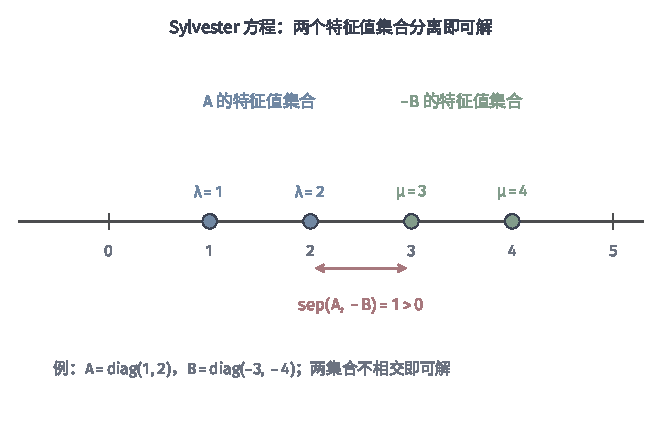
\includegraphics[width=112mm]{figures/00-shared/mathematical-preliminaries-upper/02-linear-spaces/matplotlib/ls-sylvester-separation/ls-sylvester-separation.pdf}
  \caption{Sylvester方程$\bm A\bm X+\bm X\bm B=\bm C$的特征值分离条件。
  $\bm A=\operatorname{diag}(1,2)$的特征值$\{1,2\}$与$-\bm B$（$\bm B=\operatorname{diag}(-3,-4)$）
  的特征值$\{3,4\}$分居实轴两侧，最近一对间距$|2-3|=1>0$，
  两集合不相交，故对任意$\bm C$有唯一解。只用实轴，不引入复数对象。}
  \label{fig:ls-sylvester-separation}
\end{figure}

\paragraph{Sylvester算子的可逆性}

一般情形的结论与对角情形相同。Sylvester算子$\mathcal L(\bm X)=\bm A\bm X+\bm X\bm B$可逆，当且仅当
\begin{equation}
 \lambda_i(\bm A)+\lambda_j(\bm B)\neq0
 \quad\text{对所有 }i,j,
 \qquad\text{即}\qquad
 \operatorname{spec}(\bm A)\cap\operatorname{spec}(-\bm B)=\varnothing,
 \label{eq:ch06-sylvester-spectral-separation}
\end{equation}
其中$\operatorname{spec}$表示全体特征值，包括复特征值。实矩阵的特征值可能是复数（第~\ref{sec:ls-general-square-spectrum}节），所以条件要对全体特征值检查。

证明中会用到复特征向量。这样做是允许的：$\mathcal L$可逆等价于Kronecker矩阵~\eqref{eq:ls-sylvester-vectorized}的行列式非零，
而行列式不论在实数域还是复数域中计算都是同一个数，所以在复数域中证明齐次方程只有零解，也就证明了实算子可逆。

必要性。设条件不成立，即有$\bm A\bm u=\lambda\bm u$（$\bm u\neq\bm0$），且$-\lambda$是$\bm B$的特征值。
$\bm B^\top$与$\bm B$的特征多项式相同（$\det(\bm B^\top-\mu\bm I)=\det(\bm B-\mu\bm I)$），
所以存在$\bm w\neq\bm0$使$\bm B^\top\bm w=-\lambda\bm w$，即$\bm w^\top\bm B=-\lambda\bm w^\top$。
取$\bm X=\bm u\bm w^\top$，它不是零矩阵，而
\[
 \bm A\bm X+\bm X\bm B=(\bm A\bm u)\bm w^\top+\bm u(\bm w^\top\bm B)
 =\lambda\bm u\bm w^\top-\lambda\bm u\bm w^\top=\bm0 .
\]
齐次方程有非零解，算子不可逆。

充分性。设条件成立，且$\mathcal L(\bm X)=\bm0$，要证$\bm X=\bm0$。思路是找一个多项式$q$，
使$q(\bm A)=\bm0$而$q(-\bm B)$可逆，再利用二者与$\bm X$的关系。

第一步，把$\bm X$在两侧之间“搬运”。由$\bm A\bm X=\bm X(-\bm B)$，
得$\bm A^2\bm X=\bm A\bm X(-\bm B)=\bm X(-\bm B)^2$，归纳得$\bm A^k\bm X=\bm X(-\bm B)^k$；
对各次幂作线性组合，对任意多项式$q$有$q(\bm A)\bm X=\bm X\,q(-\bm B)$。

第二步，取$q$为$\bm A$的特征多项式$p_{\bm A}(z)=\det(z\bm I-\bm A)$。由Cayley--Hamilton定理~\ref{thm:ls-cayley-hamilton}，
$p_{\bm A}(\bm A)=\bm0$。在复数域中分解$p_{\bm A}(z)=\prod_k(z-\lambda_k)$，其中$\lambda_k$取遍$\bm A$的全部特征值，则
$p_{\bm A}(-\bm B)=\prod_k(-\bm B-\lambda_k\bm I)$。由条件~\eqref{eq:ch06-sylvester-spectral-separation}，
每个$\lambda_k$都不是$-\bm B$的特征值，所以每个因子$-\bm B-\lambda_k\bm I$都可逆，$p_{\bm A}(-\bm B)$作为可逆矩阵的乘积也可逆。

合起来，$\bm X\,p_{\bm A}(-\bm B)=p_{\bm A}(\bm A)\bm X=\bm0$，右乘$p_{\bm A}(-\bm B)^{-1}$得$\bm X=\bm0$。齐次方程只有零解，算子可逆。

至此，Sylvester方程的存在性与唯一性完全由$\bm A$与$-\bm B$的特征值是否分离决定。
条件不成立时，方程对有些右端无解、对另一些右端有无穷多解，齐次解$\bm u\bm w^\top$给出了解不唯一的方向。

\subsection{求解方法}
\label{sec:ls-matrix-equation-solve}

求解方法按$\bm A$、$\bm B$的结构分两种情况。一般情况下，方程可以化为普通线性方程直接求解，
但规模大时要用实Schur形把它约化成准三角形再逐块回代；$\bm A$、$\bm B$可对角化时，换到特征向量坐标后方程按元素分开，直接写出解。

\subsubsection{一般情况}
\label{sec:ls-one-sided-two-sided}

\paragraph{向量化直接求解}

最直接的做法是形成系数矩阵~\eqref{eq:ls-sylvester-vectorized}，用第~\ref{sec:ls-direct-methods}节的LU分解求解。
小规模问题这样做是可靠的，但系数矩阵有$(mn)^2$个元素，稠密LU约需$2(mn)^3/3$次运算；
$m=n=100$时系数矩阵已有$10^8$个元素。所以要尽量利用方程的结构，避免形成这个大矩阵。

单侧和双侧方程很容易做到。$\bm A\bm X=\bm C$是同一系数矩阵的多右端问题，对$\bm A$分解一次即可逐列复用。
双侧方程在$\bm A,\bm B$可逆时，先解$\bm A\bm Y=\bm C$，再解$\bm X\bm B=\bm Y$（即$\bm B^\top\bm X^\top=\bm Y^\top$），
也不形成Kronecker矩阵。双侧方程不相容时，可以改求$\min_{\bm X}\lVert\bm A\bm X\bm B-\bm C\rVert_{\mathrm F}^2$，
它是系数矩阵为$\bm B^\top\otimes\bm A$的最小二乘问题，由第~\ref{sec:ls-least-squares}节的方法求解。
Sylvester方程的两项相加，不能这样逐侧处理，下面借助$\bm A$、$\bm B$的正交相似变换。

\paragraph{实Schur约化}
\label{sec:ls-sylvester-schur}

正交变换不放大误差，而且由第~\ref{sec:ls-general-square-spectrum}节的实Schur形（定理~\ref{thm:ls-real-schur}），
任何实方阵都可以用正交相似化为接近三角的形状：$\bm A=\bm Q\bm T\bm Q^\top$，
$\bm Q$正交，$\bm T$是实准上三角矩阵，即对角线上是$1\times1$块（实特征值）或$2\times2$块（一对共轭复特征值），
对角块以下全为零。

分别取$\bm A=\bm Q\bm T\bm Q^\top$、$\bm B=\bm U\bm S\bm U^\top$，方程两边左乘$\bm Q^\top$、右乘$\bm U$，
利用$\bm Q^\top\bm A=\bm T\bm Q^\top$与$\bm B\bm U=\bm U\bm S$，并记$\bm Y=\bm Q^\top\bm X\bm U$、$\bm D=\bm Q^\top\bm C\bm U$，方程化为
\begin{equation}
 \bm T\bm Y+\bm Y\bm S=\bm D.
 \label{eq:ls-sylvester-transformed}
\end{equation}
正交相似不改变特征值，所以可逆条件不变；正交变换也不改变Frobenius范数，所以新坐标下的残差大小与原坐标相同。

\paragraph{准三角块上的逐块回代}

$\bm T$、$\bm S$不是对角的，方程不能按元素完全分开，但三角结构允许逐块依次求解，正如上三角方程可以回代。
按$\bm T$、$\bm S$的对角块把$\bm Y$、$\bm D$分块，比较第$(i,j)$块：
$(\bm T\bm Y)_{i,j}=\sum_k\bm T_{i,k}\bm Y_{k,j}$中只有$k\geq i$的项非零，
$(\bm Y\bm S)_{i,j}=\sum_\ell\bm Y_{i,\ell}\bm S_{\ell,j}$中只有$\ell\leq j$的项非零。
把含$\bm Y_{i,j}$的两项留在左边，其余移到右边：
\begin{equation}
 \bm T_{i,i}\bm Y_{i,j}+\bm Y_{i,j}\bm S_{j,j}
 =\bm D_{i,j}-\sum_{k>i}\bm T_{i,k}\bm Y_{k,j}
          -\sum_{\ell<j}\bm Y_{i,\ell}\bm S_{\ell,j}.
 \label{eq:ls-sylvester-block-recurrence}
\end{equation}
右边只用到同一列中更靠下的块$\bm Y_{k,j}$（$k>i$）和同一行中更靠左的块$\bm Y_{i,\ell}$（$\ell<j$）。
因此按列从左到右、每列从下到上的次序计算，每次右边需要的块都已求出。左边是一个小的Sylvester方程：
两个对角块都是$1\times1$时，它就是标量方程，直接除以$t_{i,i}+s_{j,j}$；含$2\times2$块时，它至多含$4$个未知量，
向量化后系数矩阵为$\bm I\otimes\bm T_{i,i}+\bm S_{j,j}^\top\otimes\bm I$。小块的特征值是$\bm A$、$\bm B$特征值的一部分，
由谱分离条件，每个小方程都唯一可解。

全部块求出后，由$\bm X=\bm Q\bm Y\bm U^\top$恢复原坐标，并在原坐标中计算残差$\bm A\bm X+\bm X\bm B-\bm C$。这一方法称为Bartels--Stewart算法。
两次实Schur约化的代价为$O(m^3+n^3)$，逐块回代的代价为$O(mn(m+n))$，远小于向量化直接求解的$O(m^3n^3)$；
约化只做一次，多个右端$\bm C$可以复用。

\subsubsection{可对角情况}
\label{sec:ls-sylvester-diagonalizable}

若$\bm A$、$\bm B$可以对角化，逐块回代可以省去：换到特征向量坐标后，问题就是对角情形，有闭式解~\eqref{eq:ls-sylvester-diagonal-closed-form}。
设$\bm A=\bm V\bm\Lambda\bm V^{-1}$、$\bm B=\bm R\bm M\bm R^{-1}$，
其中$\bm\Lambda=\operatorname{diag}(\lambda_i)$、$\bm M=\operatorname{diag}(\mu_j)$。方程两边左乘$\bm V^{-1}$、右乘$\bm R$，
\[
 \bm V^{-1}\bm A\bm X\bm R+\bm V^{-1}\bm X\bm B\bm R=\bm V^{-1}\bm C\bm R .
\]
利用$\bm V^{-1}\bm A=\bm\Lambda\bm V^{-1}$与$\bm B\bm R=\bm R\bm M$，并记$\bm Y=\bm V^{-1}\bm X\bm R$、$\bm D=\bm V^{-1}\bm C\bm R$，得
\begin{equation}
 \bm\Lambda\bm Y+\bm Y\bm M=\bm D,
 \qquad
 y_{i,j}=\frac{d_{i,j}}{\lambda_i+\mu_j}.
 \label{eq:ls-sylvester-diagonalized}
\end{equation}
最后由$\bm X=\bm V\bm Y\bm R^{-1}$变回原坐标。分母非零恰是谱分离条件~\eqref{eq:ch06-sylvester-spectral-separation}。
下面用图~\ref{fig:ls-sylvester-separation}中的两个对角矩阵算一个具体的解。

\begin{example}[对角Sylvester方程的闭式解]
\label{ex:ls-sylvester-diagonal}
取$\bm A=\operatorname{diag}(1,2)$、$\bm B=\operatorname{diag}(-3,-4)$，$\bm C$为$2\times2$的全$1$矩阵。
两个矩阵已经是对角的，可取$\bm V=\bm R=\bm I$，于是$\bm D=\bm C$。四个分母为
\[
 1-3=-2,\qquad 1-4=-3,\qquad 2-3=-1,\qquad 2-4=-2,
\]
都不为零，由式~\eqref{eq:ls-sylvester-diagonalized}得
\[
 \bm X=\begin{bmatrix}-1/2&-1/3\\-1&-1/2\end{bmatrix}.
\]
代回可验，例如第$(1,1)$元$1\cdot(-\tfrac12)+(-\tfrac12)(-3)=1$。
\end{example}

$\bm A,\bm B$都是实对称矩阵时，特征向量可以取为标准正交的（定理~\ref{thm:ls-real-symmetric-spectral}），
此时$\bm V^{-1}=\bm V^\top$，全部计算都是实的，坐标变换也不放大误差。一般的可对角化矩阵则未必如此：
特征值可能是复数，特征向量矩阵也可能接近奇异，求逆和换坐标本身就会放大误差。
这时即使矩阵可以对角化，也宜改用一般情况的实Schur约化。

\section{李雅普诺夫方程}
\label{sec:ls-lyapunov}

Sylvester方程有一个常见的对称特例：取$\bm B=\bm A^\top$，右端记为对称矩阵$\bm Q$，得到连续型李雅普诺夫方程，即\term{Lyapunov方程}（Lyapunov equation）
\[
 \bm A\bm X+\bm X\bm A^\top=\bm Q ,\qquad \bm A,\bm Q\in\mathbb R^{n\times n},\ \bm Q=\bm Q^\top .
\]
它在线性动态系统的稳定性分析与协方差计算中经常出现，所求的$\bm X$通常应当对称，有时还要求正定。
与它对应的离散型Lyapunov方程是
\[
 \bm X-\bm A^\top\bm X\bm A=\bm Q ,
\]
它不是Sylvester方程，而是双侧作用减去恒等作用；按向量化恒等式，系数矩阵为$\bm I-\bm A^\top\otimes\bm A^\top$。
本节依次回答：方程何时唯一可解，解是否对称，怎样利用对称性求解，以及解何时正定。

\subsection{可解性与解的对称性}
\label{sec:ls-lyapunov-solvability}

连续型方程是Sylvester方程的特例，可解条件可以直接读出。$\bm A^\top$与$\bm A$的特征值相同，
由谱分离条件~\eqref{eq:ch06-sylvester-spectral-separation}，算子$\bm X\mapsto\bm A\bm X+\bm X\bm A^\top$可逆，
当且仅当对$\bm A$的任意两个（可以相同的）特征值都有$\lambda_i+\lambda_j\neq0$。
取$i=j$可见，$\bm A$有零特征值时条件不成立；有一对纯虚特征值$\pm\mathrm i\omega$时也不成立。
例如$\bm A$的全部特征值实部为负时，任意两个之和的实部也为负，条件成立。

右端$\bm Q$对称且算子可逆时，解$\bm X$自动对称。对方程两边转置，得
$\bm A\bm X^\top+\bm X^\top\bm A^\top=\bm Q^\top=\bm Q$，说明$\bm X^\top$也是解；由唯一性，$\bm X=\bm X^\top$。
这只用到唯一性，不依赖任何稳定性假设。

离散型方程的齐次形式是$\bm X=\bm A^\top\bm X\bm A$。设谱半径$\rho(\bm A)<1$，反复代入得$\bm X=(\bm A^\top)^k\bm X\bm A^k$，
而由定理~\ref{thm:ls-power-decay}，$\bm A^k\to\bm0$，所以$\bm X=\bm0$：齐次方程只有零解，方程对每个$\bm Q$唯一可解。
一般的判据是对$\bm A$的任意两个特征值都有$\lambda_i\lambda_j\neq1$，可以仿照Sylvester算子可逆性的论证证明，这里不展开。
对称性的论证与连续型相同：$\bm Q$对称时，$\bm X^\top$也是解，唯一性迫使$\bm X=\bm X^\top$。

\subsection{求解方法}
\label{sec:ls-lyapunov-solve}

连续型方程可以直接用Bartels--Stewart算法，而且因为$\bm B=\bm A^\top$，只需对$\bm A$作一次实Schur约化
$\bm A=\bm U\bm T\bm U^\top$，此时$\bm A^\top=\bm U\bm T^\top\bm U^\top$。令$\bm Y=\bm U^\top\bm X\bm U$、$\bm D=\bm U^\top\bm Q\bm U$，方程化为
\[
 \bm T\bm Y+\bm Y\bm T^\top=\bm D .
\]
与递推~\eqref{eq:ls-sylvester-block-recurrence}不同，这里右侧乘的是下三角的$\bm T^\top$：
$(\bm Y\bm T^\top)_{i,j}=\sum_\ell\bm Y_{i,\ell}\bm T_{j,\ell}^\top$中只有$\ell\geq j$的项非零。于是第$(i,j)$块满足
\[
 \bm T_{i,i}\bm Y_{i,j}+\bm Y_{i,j}\bm T_{j,j}^\top
 =\bm D_{i,j}-\sum_{k>i}\bm T_{i,k}\bm Y_{k,j}-\sum_{\ell>j}\bm Y_{i,\ell}\bm T_{j,\ell}^\top ,
\]
右边用到的是同一列中更靠下的块和同一行中更靠右的块，所以要从右下角开始，按列从右到左、每列从下到上计算。

对称性还能省去一半计算。$\bm D$对称，解$\bm Y$也对称，$\bm Y_{i,\ell}=\bm Y_{\ell,i}^\top$；按这个次序只算对角线及其下方的块，
右边需要的上方块都可以由已经算出的下方块转置得到。$n\times n$的未知量因此从$n^2$个减为$n(n+1)/2$个。
最后由$\bm X=\bm U\bm Y\bm U^\top$变回原坐标。

离散型方程同样先作约化，得$\bm Y-\bm T^\top\bm Y\bm T=\bm D$。比较第$(i,j)$块，
$(\bm T^\top\bm Y\bm T)_{i,j}=\sum_{k\leq i,\ \ell\leq j}\bm T_{k,i}^\top\bm Y_{k,\ell}\bm T_{\ell,j}$，
依赖的是行、列下标都不超过$(i,j)$的块。因此递推要从左上角开始，每一步解一个形如
$\bm Y_{i,j}-\bm T_{i,i}^\top\bm Y_{i,j}\bm T_{j,j}=\cdots$的小方程。块之间的依赖关系与连续型不同，不能照搬连续型的递推次序。

\subsection{解的正定性}
\label{sec:ls-lyapunov-positivity}

对称的解是否正定，是比可解性更强的问题。下面的充分条件都要求右端定号，并要求$\bm A$满足稳定性条件。

离散型方程在$\rho(\bm A)<1$时可以把解直接写出来。方程可以改写成$\bm X=\bm Q+\bm A^\top\bm X\bm A$，
反复代入右边的$\bm X$，就是把每步的作用$\bm X\mapsto\bm A^\top\bm X\bm A$反复施加在$\bm Q$上并累加，
这与第~\ref{sec:ls-matrix-series-exponential}节的Neumann级数同出一辙。于是考虑
\begin{equation}
 \bm X=\sum_{k=0}^{\infty}(\bm A^{\top})^k\bm Q\bm A^k .
 \label{eq:ls-discrete-lyapunov-series}
\end{equation}
取$r$满足$\rho(\bm A)<r<1$，由引理~\ref{lem:ls-power-geometric-bound}，存在常数$C_r$使$\lVert\bm A^k\rVert_2\leq C_rr^k$，
所以第$k$项的范数不超过$\lVert\bm Q\rVert_2\lVert\bm A^k\rVert_2^2\leq\lVert\bm Q\rVert_2C_r^2r^{2k}$，级数按几何级数收敛。
它满足方程：逐项计算，$\bm A^\top\bm X\bm A=\sum_{k\geq1}(\bm A^\top)^k\bm Q\bm A^k$，与$\bm X$相减只剩$k=0$项$\bm Q$。
由第~\ref{sec:ls-lyapunov-solvability}节的唯一性，级数~\eqref{eq:ls-discrete-lyapunov-series}就是方程的唯一解。

标量情形最容易核对。

\begin{example}[标量离散Lyapunov方程]
\label{ex:ls-scalar-discrete-lyapunov}
取$n=1$、$\bm A=a$、$\bm Q=q$，$|a|<1$。级数~\eqref{eq:ls-discrete-lyapunov-series}是公比为$a^2$的几何级数：
\[
 x=\sum_{k=0}^{\infty}a^{2k}q=\frac{q}{1-a^2}.
\]
代入方程，$x-a^2x=(1-a^2)\dfrac{q}{1-a^2}=q$，恰好成立。$q>0$时$x>0$，与下面的正定性结论一致。
\end{example}

这一表示直接给出正定性。若$\bm Q\succ0$，则对$\bm x\neq\bm0$，
\[
 \bm x^\top\bm X\bm x=\sum_{k=0}^{\infty}(\bm A^k\bm x)^\top\bm Q(\bm A^k\bm x)\geq\bm x^\top\bm Q\bm x>0 ,
\]
解正定；$\bm Q\succeq0$时每一项都非负，同理得$\bm X\succeq0$。

连续型的对应结论是：$\bm A$的全部特征值实部为负、右端负定，即$\bm A\bm X+\bm X\bm A^\top=-\bm W$且$\bm W\succ0$时，解$\bm X$正定。
它的证明要把解写成积分$\int_0^\infty e^{t\bm A}\bm W e^{t\bm A^\top}\,\mathrm dt$，本卷不展开。
实际计算时不必依赖这些表示：对算出的$\bm X$作Cholesky分解，分解成功即说明$\bm X\succ0$（第~\ref{sec:ls-direct-methods}节）。

\section{本章小结}
\label{sec:ls-equations-summary}

本章讨论了三个反求输入的问题：线性方程$\bm A\bm x=\bm b$、Sylvester方程$\bm A\bm X+\bm X\bm B=\bm C$与Lyapunov方程$\bm A\bm X+\bm X\bm A^\top=\bm Q$。
三者都是有限维空间上的线性方程，都先判断解的情况，再求解。

线性方程的情况由秩判别：$\operatorname{rank}[\bm A\;\bm b]=\operatorname{rank}(\bm A)$时有解，全部解是一个特解加$\operatorname{null}(\bm A)$。
唯一解按矩阵结构用LU、Cholesky或LDL$^{\top}$等直接法算出；有无穷多解时须声明准则，欧氏范数最小的解落在$\operatorname{range}(\bm A^\top)$中；
无解时改求最小二乘，残差与列空间正交给出总是相容的正规方程。伪逆把三种答案统一为$\bm A^\dagger\bm b$。
数据有误差时，条件数刻画解的放大，根源是小奇异值，形成正规方程还会把条件数平方。
岭回归与截断SVD以增加残差为代价压低或丢弃小奇异值方向；修正Gram--Schmidt、Householder反射与Givens旋转不改变问题，只让计算更稳定。

Sylvester方程对任意右端唯一可解，当且仅当$\bm A$与$-\bm B$没有公共特征值；求解时不形成Kronecker系数矩阵，而用实Schur约化后逐块回代。
Lyapunov方程是$\bm B=\bm A^\top$的特例，对称右端的解由唯一性保证对称，求解只需一次约化、只算一半的块；
离散型方程在$\rho(\bm A)<1$时有级数解，由它可读出$\bm Q\succ0$时解正定。
